\section{Results}\label{sec:results}

\begin{figure}[t]
    \centering
    \begin{subfigure}[t]{0.24\textwidth}
        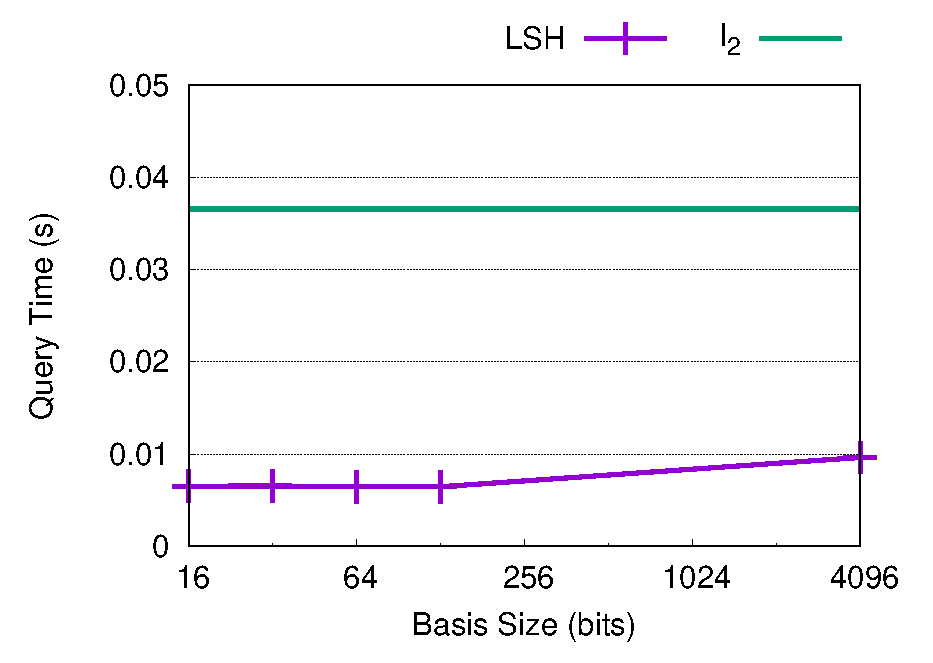
\includegraphics[width=\textwidth]{images/hashing_time_results.eps}
        \caption{Hashing query time as a function of basis size. $l_2$ speed plotted in green for comparison.}
    \end{subfigure} 
    \begin{subfigure}[t]{0.24\textwidth}
        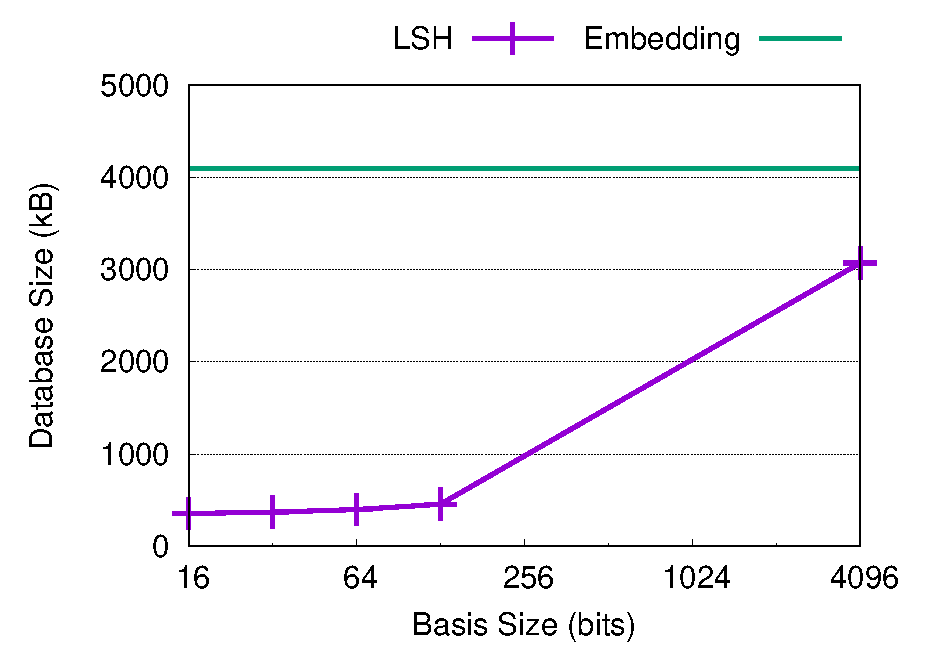
\includegraphics[width=\textwidth]{images/hashing_memory_results.eps}
        \caption{Database size as a function of basis size. Size using the embedding space plotted in green for comparison.}
    \end{subfigure}
    \caption{LSH Quantitative Results. Note that even with 4096 bits, LSH search is significantly faster and the database takes up significantly less space.}
    \label{fig:lshres}
\end{figure}

We provide an empirical study of our method using two approaches. First we test our primary task of video retrieval. This is primarily a qualitative evaluation. We show how the weights learned by our model provide a good initialization for the action recognition task with a quantitative evaluation.

\subsection{Retrieval Results}

We test several aspects of the video retrieval task. In all tests, we take the UCF101 \cite{soomro2012ucf101} training set to be our database and select a single probe video from the UCF101 test set. The videos are projected into the 128 dimensional space formed by taking the fc6 output of four six-frame stack of differences distributed uniformly at random from the video. The 128 dimensional representation for each stack of difference is averaged to give the 128 dimensional representation for each video. Our system then returns the top $n$ videos for the given probe image. We tested with $n=5$ but for brevity, only the top match is shown in the qualitative results.

Figure \ref{fig:retres} shows qualitative results of our method. Three representative probe videos were chosen for the figure that had roughly orthogonal motion types. The first video, from the "Cliff Diving" class has fast intricate motions coupled with large camera motions. The second video, from the "Bowling" class, contains constrained small motions and no camera motion. The final video, from the "Knitting" class, contains slow and highly controlled motions with the foreground occupying most of the frame. We show the top retrieval result using $l_2$ distance in the embedding space and using LSH with basis sizes of 16, 32, 64, 128, and 4096 bits. As shown in the figure, the top retrieval result correctly captures the type of motion in the probe video for $l_2$ distance. Additionally for LSH basis sizes of as small as 64 bits, the motion is still correctly captured. It is worth noting that our method does not work well on all motion types. For example, the "Knitting" class shown in the figure contains results that are qualitatively worse than the other two classes. The full retrieval results, along with videos, are provided in the supplementary material.

\begin{figure*}[t]
    \begin{center}
        \begin{tabu} to \textwidth {|X[c]|X[c]|X[c]X[c]X[c]X[c]X[c]|}
           \hline
            Probe & $l_2$ & 4096 & 128 & 64 & 32 & 16 \\ \hline \hline
            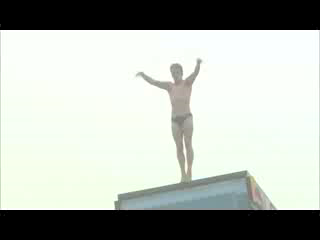
\includegraphics[width=0.1\textwidth]{images/ret_results/0/probe.png} & 
            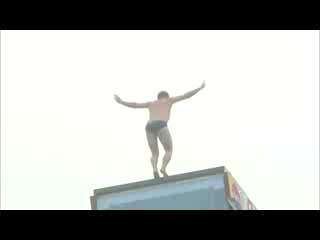
\includegraphics[width=0.1\textwidth]{images/ret_results/0/l2.png} & 
            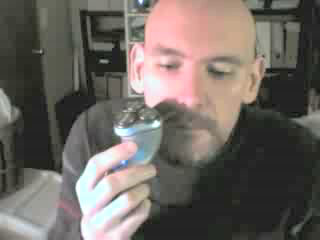
\includegraphics[width=0.1\textwidth]{images/ret_results/0/4096.png} &
            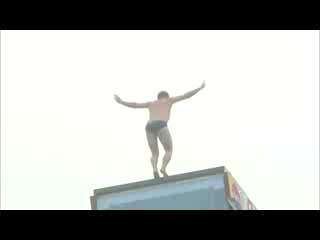
\includegraphics[width=0.1\textwidth]{images/ret_results/0/128.png} &
            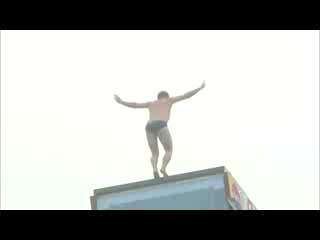
\includegraphics[width=0.1\textwidth]{images/ret_results/0/64.png} & 
            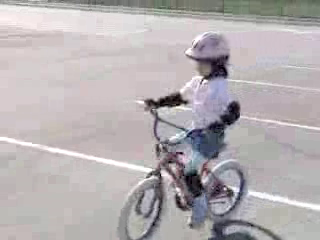
\includegraphics[width=0.1\textwidth]{images/ret_results/0/32.png} & 
            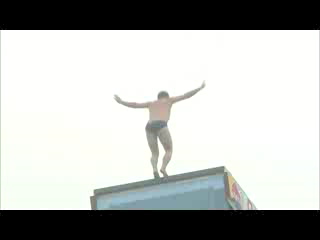
\includegraphics[width=0.1\textwidth]{images/ret_results/0/16.png} \\
            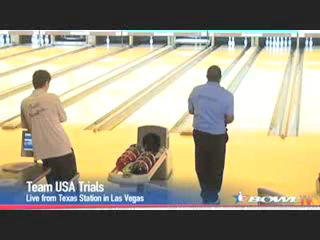
\includegraphics[width=0.1\textwidth]{images/ret_results/1/probe.png} & 
            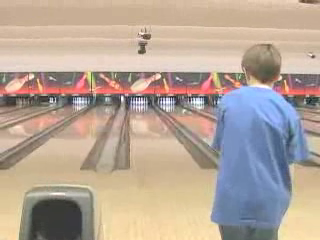
\includegraphics[width=0.1\textwidth]{images/ret_results/1/l2.png} &
            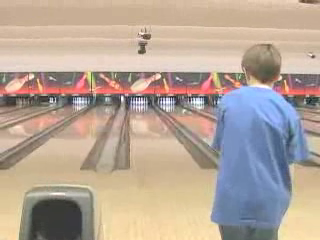
\includegraphics[width=0.1\textwidth]{images/ret_results/1/4096.png} &
            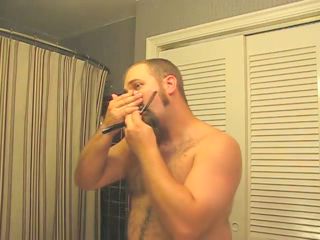
\includegraphics[width=0.1\textwidth]{images/ret_results/1/128.png} &
            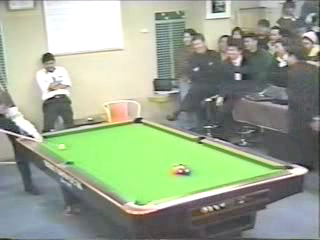
\includegraphics[width=0.1\textwidth]{images/ret_results/1/64.png} &
            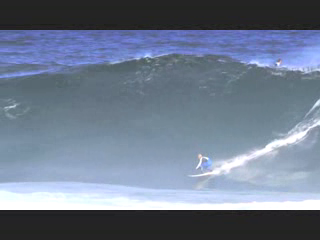
\includegraphics[width=0.1\textwidth]{images/ret_results/1/32.png} &
            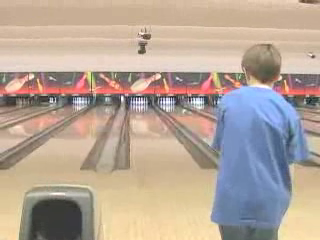
\includegraphics[width=0.1\textwidth]{images/ret_results/1/16.png} \\
            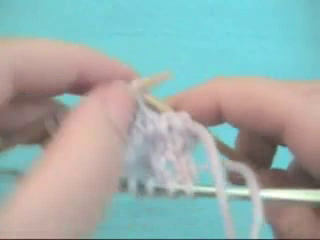
\includegraphics[width=0.1\textwidth]{images/ret_results/2/probe.png} & 
            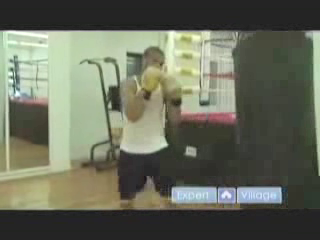
\includegraphics[width=0.1\textwidth]{images/ret_results/2/l2.png} &
            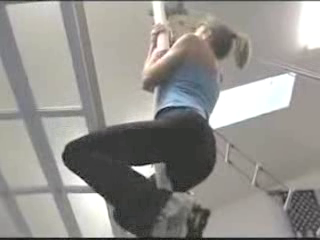
\includegraphics[width=0.1\textwidth]{images/ret_results/2/4096.png} &  
            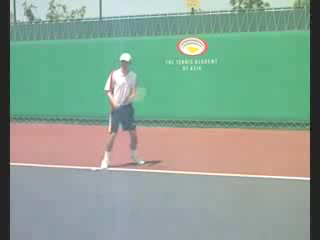
\includegraphics[width=0.1\textwidth]{images/ret_results/2/128.png} &
            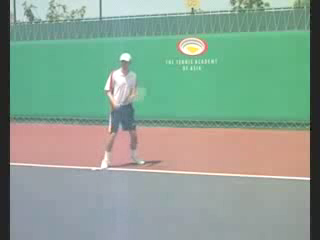
\includegraphics[width=0.1\textwidth]{images/ret_results/2/64.png} &
            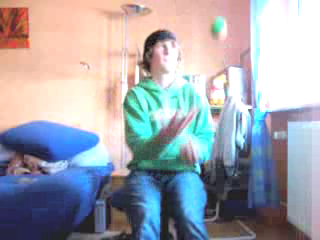
\includegraphics[width=0.1\textwidth]{images/ret_results/2/32.png} &
            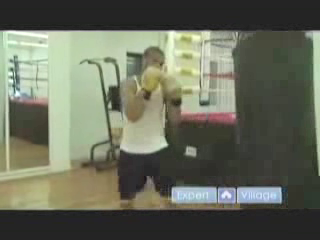
\includegraphics[width=0.1\textwidth]{images/ret_results/2/16.png} \\ \hline            
        \end{tabu}
        \caption{Qualitative retrieval results. The learned representations successfully capture similar motions in the videos. For the visualization, a single representative frame is taken from each video. The frame from the probe is shown in the left-most column. The next columns show the retrieval results for $l_2$ distance in the embedding space and for the LSH basis sizes.  }
        \label{fig:retres}
    \end{center}
\end{figure*}



\begin{figure*}[t]
    \centering
        \begin{tabu} to \textwidth {|X[c,m]|X[c,m]X[c,m]X[c,m]X[c,m]X[c,m]|}
            \hline
            Class & Biking & CliffDiving & Knitting & PizzaTossing & SkateBoarding \\ \hline \hline
            Misclassified & 
            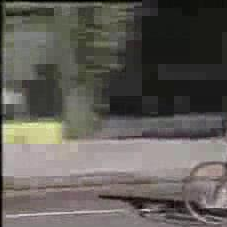
\includegraphics[width=0.1\textwidth]{images/rep/F_10.png}\vspace{2mm} & % vspace for presentation (otherwise images are clumpted together)
            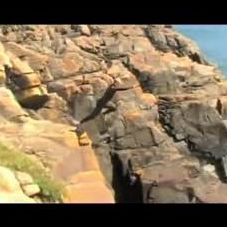
\includegraphics[width=0.1\textwidth]{images/rep/F_21.png}\vspace{2mm} &
            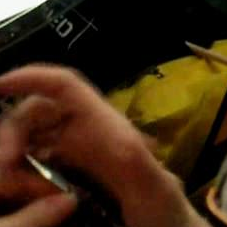
\includegraphics[width=0.1\textwidth]{images/rep/F_49.png}\vspace{2mm} & 
            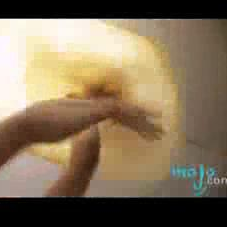
\includegraphics[width=0.1\textwidth]{images/rep/F_57.png}\vspace{2mm} &
            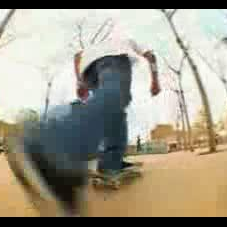
\includegraphics[width=0.1\textwidth]{images/rep/F_79.png}\vspace{2mm} \\
            Correct & 
            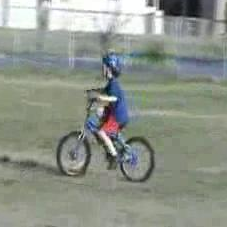
\includegraphics[width=0.1\textwidth]{images/rep/R_10.png} &
            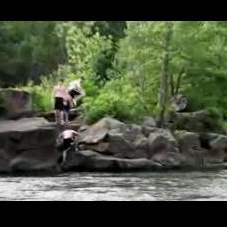
\includegraphics[width=0.1\textwidth]{images/rep/R_21.png} &
            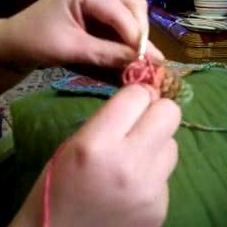
\includegraphics[width=0.1\textwidth]{images/rep/R_49.png} & 
            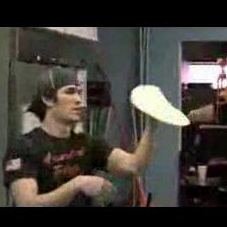
\includegraphics[width=0.1\textwidth]{images/rep/R_57.png} &
            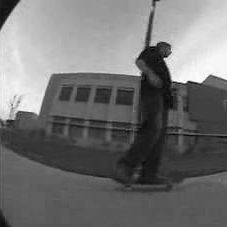
\includegraphics[width=0.1\textwidth]{images/rep/R_79.png}\\ \hline            
        \end{tabu}
        \caption{Example videos that are correctly or misclassified.}
        \label{fig:classexamples}
\end{figure*}



Next we compare the retrieval using O3N features to ours. The results are shown in Figure \ref{fig:retcomp}. We use the same procedure to produce these results as described in the first paragraph of this section, only changing the network architecture between O3N (Section \ref{sec:o3n}) and Ours (O3N with Temporal Smoothness, Section \ref{sec:network}). The top five retrieval results are given for the same "Cliff Diving" probe that was used in Figure \ref{fig:retres}. The results show that while the O3N can capture the motion type, our method does so more effectively and can even preserve the action class. While none of the O3N results are from the "Cliff Diving" class, three out of the five are in the "Cliff Diving" class for our network. Further, the second result is from the "Still Rings" class, which contains similar acrobatic movements to the "Cliff Diving" videos. More O3N retrieval results are included in the supplementary material.

Finally, we show the quantitative effect of LSH on the system speed and memory usage in Figure \ref{fig:lshres}. For these results, the same set of LSH bases, 16, 32, 64, 128, and 4096, are used. The time to retrieve the top $n=5$ videos is computed and the total storage size of the database is reported. As the results show, LSH even with a basis size of 4096 has a significant impact on the speed of retrieval and on the size of the database. Cross referencing with Figure \ref{fig:retres}, this added efficiency comes with minimal cost in the accuracy of the retrieval results. Even at a basis size of 4096 bits, the LSH database takes up approximately one third less memory than the original database and executes queries approximately four times as quickly.

\begin{table}
    \centering
    \begin{tabu} to 0.5\textwidth {|X[l]|X[c]|}
        \hline
        Initialization & Accuracy (\%) \\ \hline \hline
        ImageNet & \textbf{66.836} \\ \hline
        O3N & 52.756 \\ \hline
        Ours (O3N + TS) & 54.072 \\ \hline
    \end{tabu}
    \caption{Fine-tuned classification accuracy for different weight initializations.}
    \label{fig:classres}
\end{table}

\subsection{Classification Accuracy Results}

We also conduct a short quantitative study by using our weights as the initialization for action recognition and fine-tuning. We follow the fine-tuning procedure in \cite{fernando2017self} for both the original O3N network and for our dual-loss architecture. The results are shown in \ref{fig:classres}, our networks weights give an improvement of around 2\% over O3N initialization.

We briefly review the fine-tuning procedure. We start with the standard AlexNet network. The convolutional layers are initialized with our weights. The fully connected layers, which now have 4096 activations, are initialized with random weights. The network is then trained for the action recognition task by using a $10^{-4}$ learning rate for the convolutional layers , which should already have reasonable weights according to our hypothesis. The fully-connected layers are trained with a $10^{-2}$ learning rate since they start with random weights. 

We tested multiple different initializations to ensure a good comparison. We follow the fine-tuning procedure described above starting from ImageNet supervised weights, O3N alone, and ours (O3N with temporal smoothness). Adding the smoothness loss gives increased accuracy over using O3N alone. As expected, the ImageNet weights perform better than both of the self-supervised weights. It is worth noting that producing ImageNet weights is very expensive: it requires a much longer training process and requires labeled data. 

%XS: I temporarily comment this because both o3/4.png and smooth/4.png do not exit
\iffalse
\begin{figure*}[t]
    \centering
        \begin{tabu} to \textwidth {|X[c,m]|X[c,m]X[c,m]X[c,m]X[c,m]X[c,m]|}
            \hline
            Method & 0 & 1 & 2 & 3 & 4 \\ \hline \hline
            O3N & 
            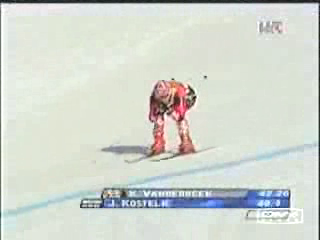
\includegraphics[width=0.1\textwidth]{images/o3vsmooth/o3/0.png}\vspace{2mm} & % vspace for presentation (otherwise images are clumpted together)
            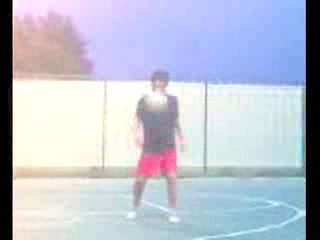
\includegraphics[width=0.1\textwidth]{images/o3vsmooth/o3/1.png}\vspace{2mm} &
            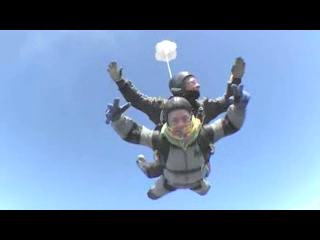
\includegraphics[width=0.1\textwidth]{images/o3vsmooth/o3/2.png}\vspace{2mm} & 
            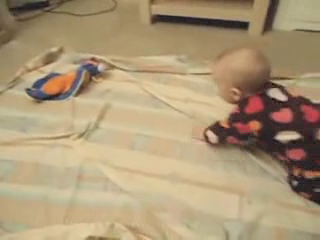
\includegraphics[width=0.1\textwidth]{images/o3vsmooth/o3/3.png}\vspace{2mm} &
            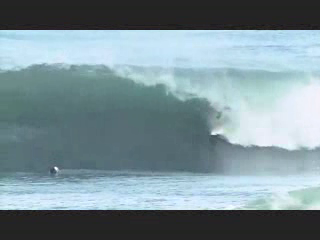
\includegraphics[width=0.1\textwidth]{images/o3vsmooth/o3/4.png}\vspace{2mm} \\
            Ours (O3N + TS) & 
            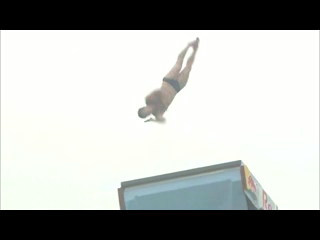
\includegraphics[width=0.1\textwidth]{images/o3vsmooth/smooth/0.png} &
            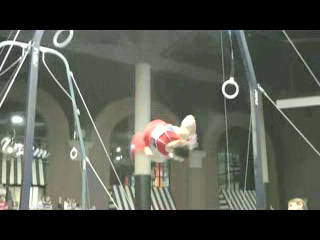
\includegraphics[width=0.1\textwidth]{images/o3vsmooth/smooth/1.png} &
            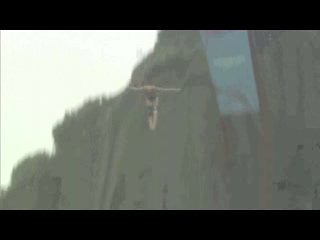
\includegraphics[width=0.1\textwidth]{images/o3vsmooth/smooth/2.png} & 
            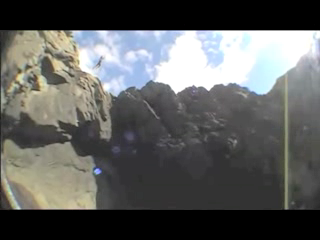
\includegraphics[width=0.1\textwidth]{images/o3vsmooth/smooth/3.png} &
            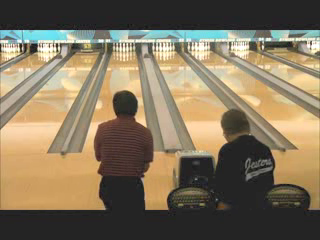
\includegraphics[width=0.1\textwidth]{images/o3vsmooth/smooth/4.png}\\ \hline            
        \end{tabu}
        \caption{Qualitative comparison, O3N vs Ours. The top five retrieval results for the same probe video for the "Cliff Diving" class in Figure \ref{fig:retres} are shown. Our method captures motion type more effectively and can preserve action class.}
        \label{fig:retcomp}
\end{figure*}
\fi

